\section{信号与系统}

    \subsection{一维信号的表示}

        \begin{description}
            \item[连续信号] 用$t$表示连续的时间自变量: $x(t)$
            \item[离散信号] 用$n$表示时间自变量: $x(n)$ or $x[n]$
        \end{description}

    \subsection{信号的能量与功率}

        \subsubsection{连续时间信号的能量和功率}

        连续时间信号$x(t)$在$t_1\leqslant t\leqslant t_2$区间的\textbf{能量}定义为
        \[ E=\int_{t_1}^{t_2}|{x(t)}|^2\d t \]
        \textbf{平均功率}定义为
        \[ P=\frac{1}{t_2-t_1}\int_{t_1}^{t_2}|x(t)|^2\d t \]
        其中, $x(t)$为复函数.

        \subsubsection{离散时间信号的能量和功率}

        离散时间信号在$n_1\leqslant n\leqslant n_2$区间的\textbf{能量}定义为
        \[ E=\sum_{n=n_1}^{n_2}|x[n]|^2 \]
        \textbf{平均功率}为
        \[ P=\frac{1}{n_2-n_1+1}\sum_{n=n_1}^{n_2}|x[n]|^2 \]

        \subsubsection{无限区间上信号的能量和功率}

        \begin{table}[h]\centering
            \caption{无限区间上信号的能量和功率}
            \label{tab:2:universal-energy-and-power}
            \begin{tabular}{ccc} \toprule
                & 连续时间信号 & 离散时间信号 \\ \midrule
                总能量 & $ E_\infty=\lim_{T\to \infty}\int_{-T}^T|x(t)|^2\d t=\int_{-\infty}^\infty|x(t)|^2\d t $ & $E_\infty=\lim_{N\to \infty}\sum_{-N}^N|x[n]|^2=\sum_{-\infty}^\infty|x[n]|^2$\\ 
                平均功率 & $P_\infty=\lim_{T\to \infty}\frac{1}{2T}\int_{-T}^T|x(t)|^2\d t$ & $P_\infty=\lim_{N\to \infty}\frac{1}{2N+1}\sum_{-N}^N|x[n]|^2$ \\ \bottomrule
            \end{tabular}
        \end{table}

        \subsubsection{三类重要信号}
        
        \begin{itemize}
            \item \textbf{能量信号} 总能量有限: $E_\infty<\infty, P_\infty=0$
            \item \textbf{功率信号} 总能量无限, 平均能量有限: $E_\infty=\infty, 0<P_\infty<\infty$
            \item 总能量和平均功率都是无限的: $E_\infty=\infty, P_\infty=\infty$ \\
                这个世界上不存在
        \end{itemize}

    \subsection{信号的自变量变换}

        \subsubsection{时移变换}

            \[x(t)\to x(t-t_0)\]

            信号向右平移$t_0$.

        \subsubsection{反转变换}

            \[x(t)\to x(-t)\]

            信号以$t=0$为轴反转.

        \subsubsection{尺度变换}

            \[x(t)\to x(at)\]

            $a>1$时, $x(at)$是将$x(t)$在时间上压缩. $0<a<1$时, $x(at)$是将$x(t)$在时间上扩展.

            \paragraph{离散信号的抽取}

                离散信号的尺度变换表现为对离散信号的抽取.

                \begin{figure}[h]\centering
                    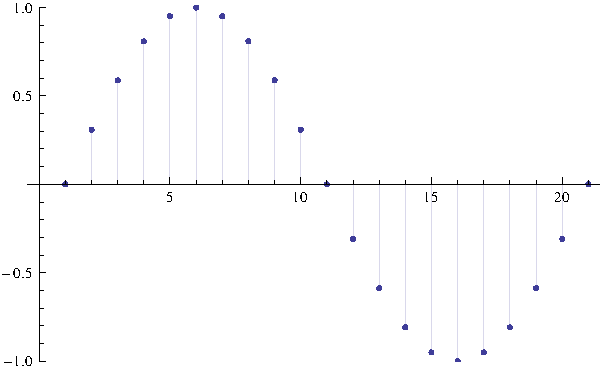
\includegraphics[width=6cm]{signals_notes/chap1_inc/dt-time-shift-o.pdf} \raisebox{1.8cm}{$\to$} 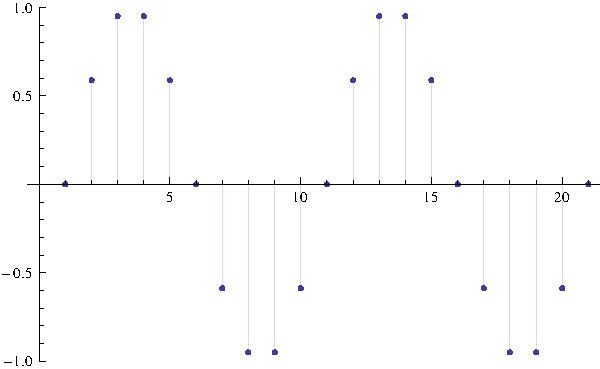
\includegraphics[width=6cm]{signals_notes/chap1_inc/dt-time-shift-a.pdf}
                    \caption{$\sin[0.1n\pi]$和$\sin[0.2n\pi]$}
                    \label{fig:2:dt-time-shift-example}
                \end{figure}

        \subsubsection{综合}

            $x(t)\to x(\alpha t+\beta)$的一般过程:
            \begin{enumerate}
                \item 首先根据$\beta$的值将$x(t)$延时或超前(平移);
                \item 根据$\alpha$的值对延时或超前的信号做尺度变换;
                \item 如果$\alpha<0$则做时间反转;
                \item 用特殊点(零点, 端点和节点)验证.
            \end{enumerate}

    \subsection{信号的周期性和奇偶性}

        \subsubsection{周期信号}

            \textbf{周期信号}满足对于全部的$t$或$n$, 存在$T\neq 0$或者$N\neq 0$使得$x(t)=x(t+T)$或者$x[n]=x[n+N]$成立, 其中$T$或$N$称为信号的\textbf{周期}.

            $2T, 3T, 4T,\cdots$或$2N, 3N, 4N, \cdots$也是信号的周期. 满足此关系的正实数(正整数)中最小的一个称为信号的\textbf{基波周期}, 表示为$T_0$或$N_0$.

            $x(t)=C$可以视为周期信号, 但基波周期没有明确的定义. $x[n]$的基波周期$N_0=1$.

        \subsubsection{信号的奇偶性}

            满足$x(-t)=x(t)$的信号是\textbf{偶信号}; 满足$x(-t)=-x(t)$的信号是\textbf{奇信号}.

            \paragraph{一个神奇的规律}

                任何信号都能分解成一个偶信号与一个奇信号之和:

                \[x(t)=x_e(t)+x_o(t)\]
                \[x_e(t)=\frac{1}{2}[x(t)+x(-t)]\]
                \[x_o(t)=\frac{1}{2}[x(t)-x(-t)]\]

    \subsection{几种基本信号}

        \subsubsection{正弦信号(Sine Wave, or sinusoid)}

            一般的正弦信号:
            \[x(t)=A\cos(\omega_0t+\phi)=\frac{A}{2}\e^{j\phi}\e^{j\omega_0t}+\frac{A}{2}\e^{-j\phi}\e^{-j\omega_0t} \]
            它的总能量是无限的, 平均功率
            \[P_\infty =\lim_{T\to\infty}\frac{1}{2T}\int_{-T}^T|\e^{j\omega_0t}|^2\d t=1\]
            因此, 周期信号是功率信号.

            \paragraph{思考题}
            
                证明周期信号都是功率信号.

        \subsubsection{连续时间指数信号}

            \[x(t)=C\e^{at}\]

            \paragraph{实指数信号}

                若$c$和$a$均为实常数, 则$x(t)$为\textbf{实指数信号}. $a>0$时单调上升, $a<0$时单调下降.

            \paragraph{周期性复指数信号}

                令$a=j\omega_0$, $C$为实数, 取$C=1$, 则
                \[x(t)=\e^{j\omega_0t}=\cos\omega_0t+j\sin\omega_0t\]
                它的实部和虚部是正弦信号.

                \begin{figure}[h]\centering
                    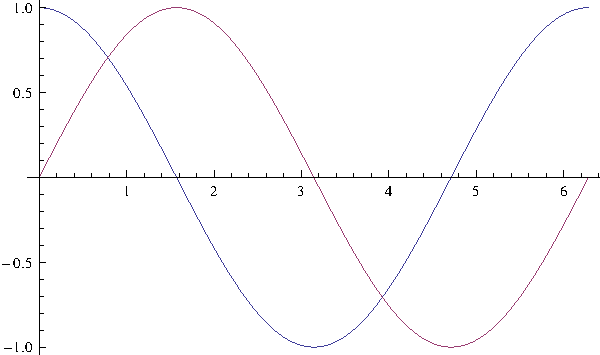
\includegraphics[width=8cm]{signals_notes/chap1_inc/euler.pdf}
                    \caption{$e^{jt}$在$[0, 2\pi]$上的实部和虚部分}
                    \label{fig:2:euler}
                \end{figure}

                显然可证$x(t)$是周期性的\footnote{用定义}, 其基波周期$T_0=\frac{2\pi}{|\omega_0|}$, 基波频率为$\omega_0$.

                令集合$\phi_k(t)=\{e^{jk\omega_0t}\}, k=0, \pm1, \pm2, \cdots$, 该信号集中的每个信号都是周期的, 它们的频率都是$\omega_0$的整数倍, 它们\textbf{成谐波关系}, 构成\textbf{完备正交基}\footnote{明神笑了}, 集合$\phi_k(t)$也称为连续时间信号的\textbf{基函数集}, 它的相关系数$\rho_{xy}=\int_{-\infty}^{\infty}x(t)y^*(t)\d t=0$\footnote{$y^*(t)$为$y(t)$的共轭}.

            \paragraph{一般连续时间复指数信号}

                在$x(t)=C\e^{at}$中, 令$C=|C|\e^{j\omega}, a=r+j\omega+0$, 则
                \[x(t)=|C|\e^{j\omega}\e^{rt}\e^{j\omega_0t}=|C|\e^{rt}\e^{j(\omega_0t+\theta)}=|C|\e^{rt}\cos(\omega_0t+\theta)+j|C|\e^{rt}\sin(\omega_0t+\theta)\]
                该信号可看成是振幅按实指数信号规律变化的复指数信号, 它的实部与虚部都是振幅呈实指数规律变化的正弦振荡.

                \begin{figure}[h]\centering
                    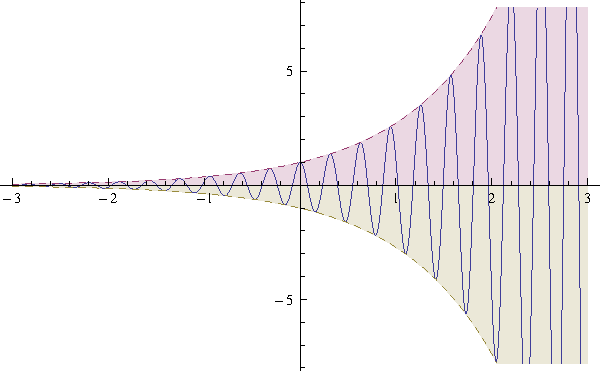
\includegraphics[width=8cm]{signals_notes/chap1_inc/compsignal.pdf}
                    \caption{$\e^t\cos(20t)$在[-3,3]上的图像}
                    \label{fig:2:comp-signal}
                \end{figure}

                \begin{itemize}
                    \item $r>0$时, 是指数增长的正弦振荡;
                    \item $r<0$时, 是指数衰减的正弦振荡;
                    \item $r=0$时, 是等幅的正弦振荡.
                \end{itemize}
            
            \paragraph{离散时间复指数信号}

                在$x[n]=C\alpha ^n$(其中$C$和$\alpha $一般为复数)中, 令$\alpha =\e^\beta $, 则有
                \[x[n]=C\e^{\beta n}\]

                若$C$和$\alpha$均取实数, 则称为\textbf{实指数序列}.

                \begin{figure}[h]\centering
                    \begin{minipage}{0.4\linewidth}\centering
                        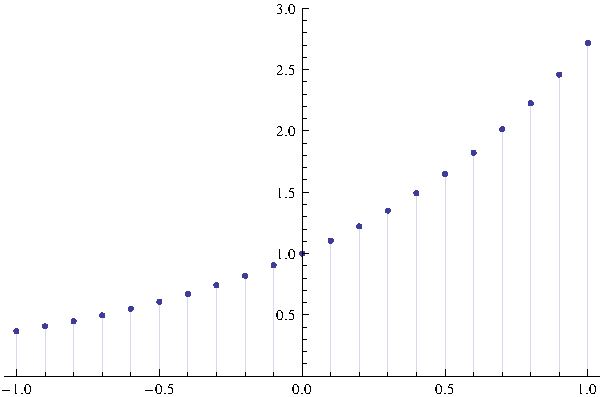
\includegraphics[width=0.8\linewidth]{signals_notes/chap1_inc/dt-sample-a.pdf}\\
                        (a) $\alpha>1$
                    \end{minipage}
                    \begin{minipage}{0.4\linewidth}\centering
                        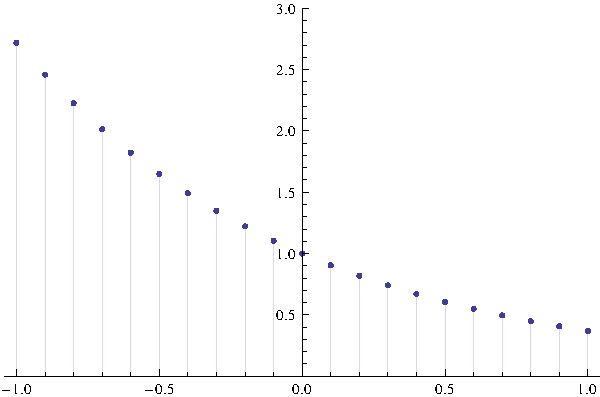
\includegraphics[width=0.8\linewidth]{signals_notes/chap1_inc/dt-sample-b.pdf}\\
                        (b) $0<\alpha<1$
                    \end{minipage}\\\
                    \begin{minipage}{0.4\linewidth}\centering
                        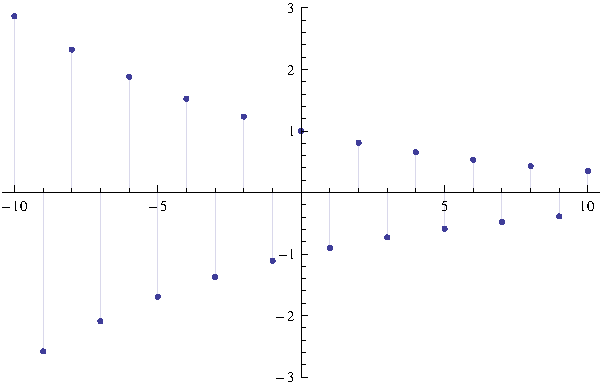
\includegraphics[width=0.8\linewidth]{signals_notes/chap1_inc/dt-sample-c.pdf}\\
                        (c) $-1<\alpha<0$
                    \end{minipage}
                    \begin{minipage}{0.4\linewidth}\centering
                        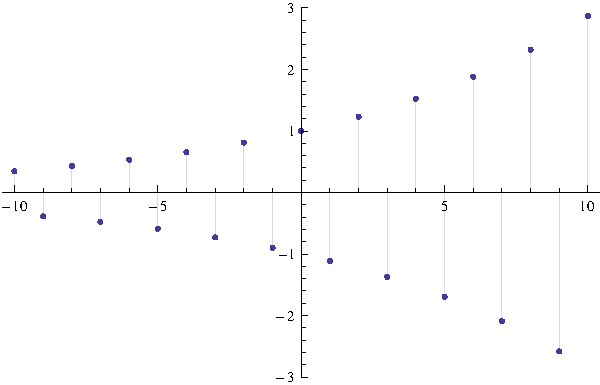
\includegraphics[width=0.8\linewidth]{signals_notes/chap1_inc/dt-sample-d.pdf}\\
                        (d) $\alpha<-1$
                    \end{minipage}\\
                    \caption{实指数序列}
                    \label{fig:2:dt-comp-singals}
                \end{figure}

                若$\alpha=\e^{j\omega}$, $C$取1, 则
                \[x[n]=\e^{j\omega_n}=\cos\omega_0n+j\sin\omega_0n\]
                它的实部和虚部都是正弦信号. 
                \[E_\infty=\lim_{N\to\infty}\sum_{n=-N}^N|\e^{j\omega_0k}|^2=\infty\]
                \[P_\infty=|\e^{j\omega_0n}|^2=1\]
                它具有无限的总能量和有限的平均功率, 恒模的复指数信号是功率信号.

                \begin{figure}[h!]\centering
                    \begin{minipage}{0.3\linewidth}\centering
                        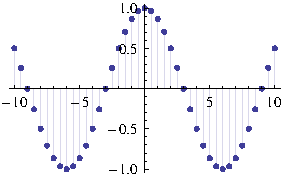
\includegraphics[width=\linewidth]{signals_notes/chap1_inc/const-dt-eg-1.pdf}\\
                        (a) $x[n]=\cos(2\pi n/12)$
                    \end{minipage}
                    \begin{minipage}{0.3\linewidth}\centering
                        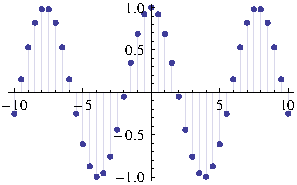
\includegraphics[width=\linewidth]{signals_notes/chap1_inc/const-dt-eg-2.pdf}\\
                        (b) $x[n]=\cos(8\pi n/31)$
                    \end{minipage}
                    \begin{minipage}{0.3\linewidth}\centering
                        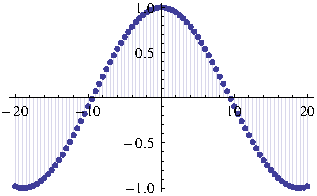
\includegraphics[width=\linewidth]{signals_notes/chap1_inc/const-dt-eg-3.pdf}\\
                        (c) $x[n]=\cos(n/6)$
                    \end{minipage}\\
                    \caption{恒模的复指数信号的实部或虚部}
                    \label{fig:2:const-dt-egs}
                \end{figure}

                若$x[n]=C\alpha^n$中的$C$和$\alpha$为复数, 则称为\textbf{一般离散时间复指数信号}. 令$C=|C|\e^{j\theta}, \alpha=|\alpha|\e^{j\omega_0}$, 则
                \[x[n]=|C||\alpha|^n\cos(\omega_0n+\theta)+j|C||\alpha|^n\sin(\omega_0n+\theta)\]

                当$|\alpha|=1$时它的实部与虚部都是正弦序列, $|\alpha|>1$时它的实部与虚部都是指数增长的正弦序列, $|\alpha|<1$时它的实部与虚部都是指数衰减的正弦序列.

                思考题: 离散时间正弦信号是否都为周期信号?

                \hfill \begin{rotate}{180}
                    因此只有在$\omega_0\over2\pi$是有理数时, 信号$\e^{j\omega_0n}$才具有周期性
                \end{rotate}

                \hfill \begin{rotate}{180}
                    $\e^{j\omega_0[n+N]}=\e^{j\omega_0n}\Leftrightarrow \e^{j\omega_0N}=1\Leftrightarrow\omega_0N=2\pi m\Leftrightarrow\frac{\omega_0}{2\pi}=\frac{m}{M}$
                \end{rotate}

                \hfill \begin{rotate}{180}
                    离散时间恒模复指数信号为周期信号的充要条件: \\
                \end{rotate} \vskip 1em

                满足周期性要求的情况下, 总能找到互素的$m>0, N>0$使得$\frac{\omega_0}{2\pi}=\frac{m}{N}$, 其中的$N=\frac{2\pi}{\omega_0}$为信号的周期, $N$称为基波周期, 因此该信号的基波频率$\omega=\frac{2\pi}{N}=\frac{\omega_0}{m}$.

                离散时间复指数序列频率具有周期性:
                \[\e^{j(\omega_0+2\pi)}=\e^{j2\pi n}\e^{j\omega_0n}=\e^{j\omega_0n}\]
                离散时间复指数信号在频率$\omega_0+2\pi$和频率$\omega_0$时是完全一样的. 因此离散时间周期性复指数信号也构成成谐波关系的信号集:
                \[\phi_k[n]=\{\e^{jk\frac{2\pi}{N}n}\}, k=0, \pm1, \pm2, \cdots\]
                该信号集中只有$N$个互不相同的信号.

                \begin{table}[h]\centering
                    \caption{比较$\e^{j\omega_0t}$和$\e^{j\omega_0n}$}
                    \label{tab:2:comparing-ct-dt}
                    \begin{tabular}{cc}\toprule
                        \bf $\e_{j\omega_0t}$ & \bf $\e_{j\omega_0n}$ \\ \midrule
                        不同频率, 信号不同 & 频率相差$2\pi$的整数倍时信号相同 \\
                        对任何频率信号都是周期的 & 仅当$\omega_0=2\pi m/N$时信号才是周期的 \\
                        基波频率为$\omega_0$ & 基波频率为$\omega_0/m$ \\
                        基波周期$T_0=2\pi/\omega_0$ & 基波周期$N_0=2\pi m/\omega_0$ \\
                        \bottomrule
                    \end{tabular}
                \end{table}

                例: 确定如下离散时间信号的基波周期:
                \[x[n]=\e^{j\frac{2\pi}{3}n}+\e^{j\frac{3\pi}{4}n}\]
